\documentclass[50pt]{article}
\usepackage[utf8]{inputenc}
\usepackage[spanish]{babel}
\usepackage[margin=2.5cm]{geometry}
\usepackage{amsmath,amssymb}
\usepackage{graphicx}
\usepackage{float}
\usepackage{enumitem}
\usepackage{listings}
\usepackage{longtable}
\usepackage{array}
\usepackage{booktabs}

\title{
    \vspace{-2.5cm} 
    {\centering 
\includegraphics[width=1.0\textwidth]{banner.png} \\[1cm]}
    \textbf{Funciones escalares de varias variables} \\[1cm]
    \large E.D. 1.1. Ejercicios \\[4cm]
}  

\author{
    253110213 - Flores Soria Ximena \\
    253110111 - Martinez Castillo Dair \\
    253110169 - Garduño Reyes Alejandro \\
    253110012 - Alvarado Villegas Gael Salvador \\
    253110534 - Belmontes Flores Joshua Shadai \\[4cm]
}

\date{Septiembre, 2026}

\begin{document}
\maketitle
\begin{center}
    \vspace{1cm}
    
    \textbf{GRUPO:} TID-401 \\[0.8cm]
    
    \textbf{Docente:} Rubén Ramírez Gómez

\end{center}


\newpage

\section{Tabla de anatomía matemática}
\begin{small}
\begin{longtable}{@{}L{2.3cm}L{3cm}cL{6cm}@{}}
\toprule
\textbf{Parte} & \textbf{Superficie} & \textbf{Centro/vértice} & \textbf{Ecuación trasladada}\\
\midrule\endhead
Suelo & Plano & -- & $z=0$\\
Pared de fondo & Plano & -- & $y=-3$\\
Pelvis/falda & Paraboloide elíptico & $(0,0,1.5)$ & $z=1.5-\dfrac{x^2+y^2}{2}$, $0\le z\le1$\\[6pt]
Torso & Hiperboloide de 1 hoja & $(0,0,2)$ & $x^2+y^2-\dfrac{(z-2)^2}{2}=0.5$, $1\le z\le3$\\[6pt]
Cinturón & Cilindro circular & $(0,0,2)$ & $x^2+y^2=0.5625$, $1.9\le z\le2.1$\\
Hombros & Cono circular & $(0,0,5)$ & $x^2+y^2=\dfrac{(z-5)^2}{4}$, $3\le z\le4$\\[6pt]
Cuello & Cilindro circular & $(0,0,4.25)$ & $x^2+y^2=0.25$, $4\le z\le4.5$\\
Cabeza & Elipsoide & $(0,0,5)$ & $x^2+y^2+\dfrac{(z-5)^2}{0.5}=1$\\[6pt]
Brazo der. & Cilindro (eje $x$) & $(1.5,0,3.5)$ & $y^2+(z-3.5)^2=0.09$, $0.5\le x\le2.5$\\
Brazo izq. & Cilindro (eje $x$) & $(-1.5,0,3.5)$ & $y^2+(z-3.5)^2=0.09$, $-2.5\le x\le-0.5$\\
Mano der. & Elipsoide & $(2.7,0,3.5)$ & $\dfrac{(x-2.7)^2}{0.25}+\dfrac{y^2}{0.1225}+\dfrac{(z-3.5)^2}{0.1225}=1$\\[6pt]
Mano izq. & Elipsoide & $(-2.7,0,3.5)$ & $\dfrac{(x+2.7)^2}{0.25}+\dfrac{y^2}{0.1225}+\dfrac{(z-3.5)^2}{0.1225}=1$\\[6pt]
Ojo der. & Elipsoide (esfera) & $(0.35,0.89,5.2)$ & $(x-0.35)^2+(y-0.89)^2+(z-5.2)^2=0.0144$\\
Ojo izq. & Elipsoide (esfera) & $(-0.35,0.89,5.2)$ & $(x+0.35)^2+(y-0.89)^2+(z-5.2)^2=0.0144$\\
Nariz & Cono circular (eje $y$) & $(0,1.3,5)$ & $x^2+(z-5)^2=\dfrac{(y-1.3)^2}{4}$, $0.9\le y\le1.3$\\[6pt]
Sombrero & Cono circular & $(0,0,7)$ & $x^2+y^2=\dfrac{(z-7)^2}{4}$, $5.4\le z\le7$\\
\bottomrule
\end{longtable}
\end{small}
 
\textbf{Ensamble.} Las piezas se tocan: en $z=1$ pelvis y torso tienen $r=1$; en $z=3$ torso y hombros tienen $r=1$; en $z=4$ hombros y cuello tienen $r=0.5$; el cuello entra en la cabeza; los brazos entran en los hombros y en las manos; los ojos, la nariz y el sombrero quedan parcialmente dentro de la cabeza.
 
\section{Construcción en GeoGebra 3D}
\begin{lstlisting}
z=0
y=-3
x^2+y^2+(z-5)^2/0.5=1
(x-2.7)^2/0.25+y^2/0.1225+(z-3.5)^2/0.1225=1
(x+2.7)^2/0.25+y^2/0.1225+(z-3.5)^2/0.1225=1
(x-0.35)^2+(y-0.89)^2+(z-5.2)^2=0.0144
(x+0.35)^2+(y-0.89)^2+(z-5.2)^2=0.0144
Surface(0.5cos(u), 0.5sin(u), v, u, 0, 2π, v, 4, 4.5)
Surface((5-v)/2 cos(u), (5-v)/2 sin(u), v, u, 0, 2π, v, 3, 4)
Surface(sqrt(0.5+(v-2)^2/2) cos(u), sqrt(0.5+(v-2)^2/2) sin(u), v, u, 0, 2π, v, 1, 3)
Surface(sqrt(3-2v) cos(u), sqrt(3-2v) sin(u), v, u, 0, 2π, v, 0, 1)
Surface(0.75cos(u), 0.75sin(u), v, u, 0, 2π, v, 1.9, 2.1)
Surface(v, 0.3cos(u), 3.5+0.3sin(u), u, 0, 2π, v, 0.5, 2.5)
Surface(v, 0.3cos(u), 3.5+0.3sin(u), u, 0, 2π, v, -2.5, -0.5)
Surface((7-v)/2 cos(u), (7-v)/2 sin(u), v, u, 0, 2π, v, 5.4, 7)
Surface((1.3-v)/2 cos(u), v, 5+(1.3-v)/2 sin(u), u, 0, 2π, v, 0.9, 1.3)
\end{lstlisting}
 
\begin{figure}[H]
\centering
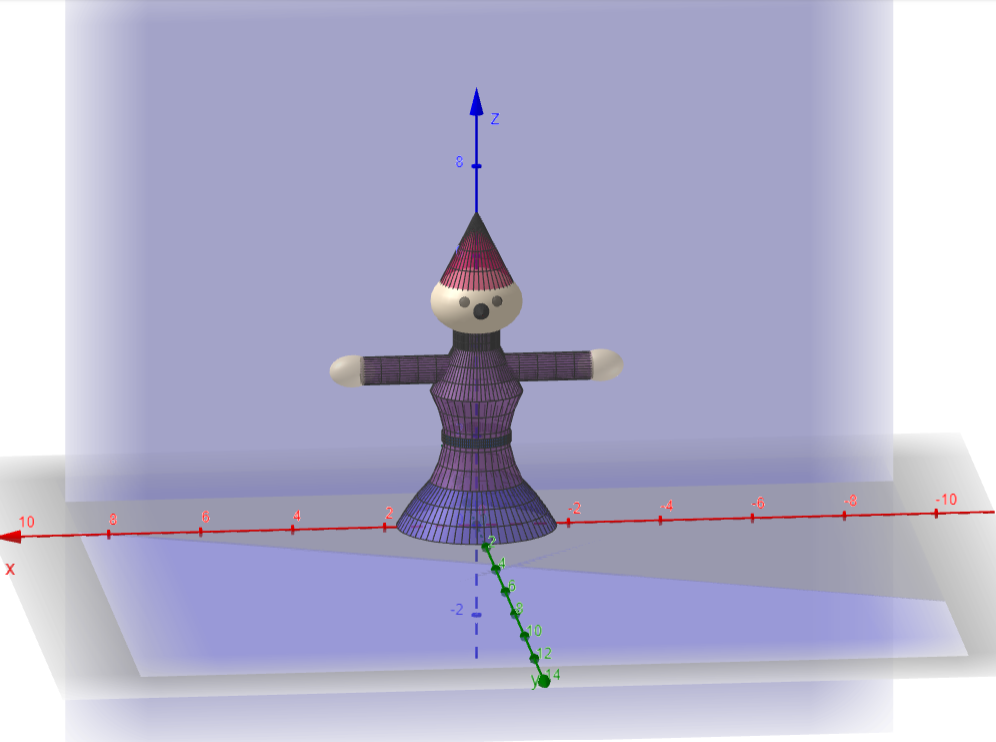
\includegraphics[width=0.48\textwidth]{vistaGeneral.png}\hfill
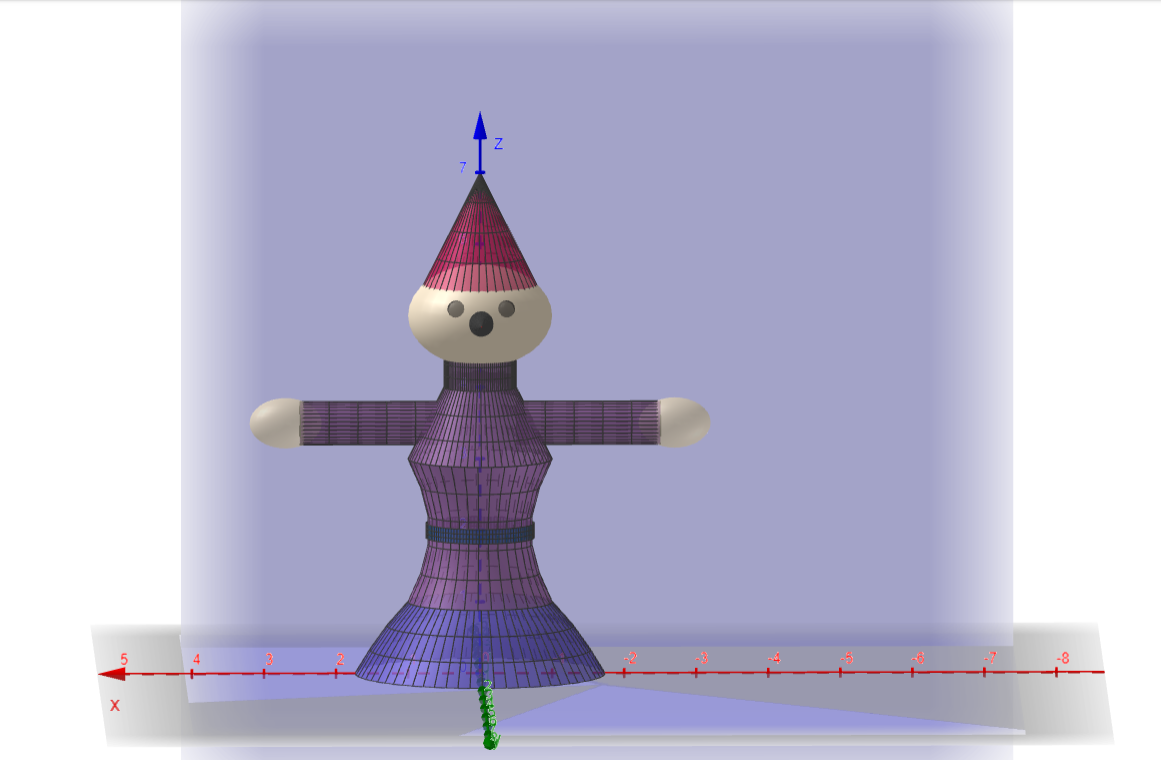
\includegraphics[width=0.48\textwidth]{vistaFrontall.png}
\caption{Vista general y vista frontal de la escultura.}
\end{figure}
 
\section{Análisis de corte}
Se creó el plano $z=k$ con un deslizador $k$ y se obtuvo la intersección con cada pieza.
 
\begin{table}[H]
\centering\renewcommand{\arraystretch}{1.5}
\begin{tabular}{@{}llc@{}}
\toprule
\textbf{Pieza} & \textbf{Curva de nivel en $z=k$} & \textbf{Tipo}\\
\midrule
Torso & $x^2+y^2=0.5+\dfrac{(k-2)^2}{2}$ & Círculo\\
Cabeza & $x^2+y^2=1-\dfrac{(k-5)^2}{0.5}$ & Círculo\\
Hombros & $x^2+y^2=\dfrac{(k-5)^2}{4}$ & Círculo\\
Sombrero & $x^2+y^2=\dfrac{(k-7)^2}{4}$ & Círculo\\
Pelvis & $x^2+y^2=3-2k$ & Círculo\\
Mano ($k=3.5$) & $\dfrac{(x-2.7)^2}{0.25}+\dfrac{y^2}{0.1225}=1$ & Elipse\\
\bottomrule
\end{tabular}
\end{table}
 
\begin{figure}[H]
\centering
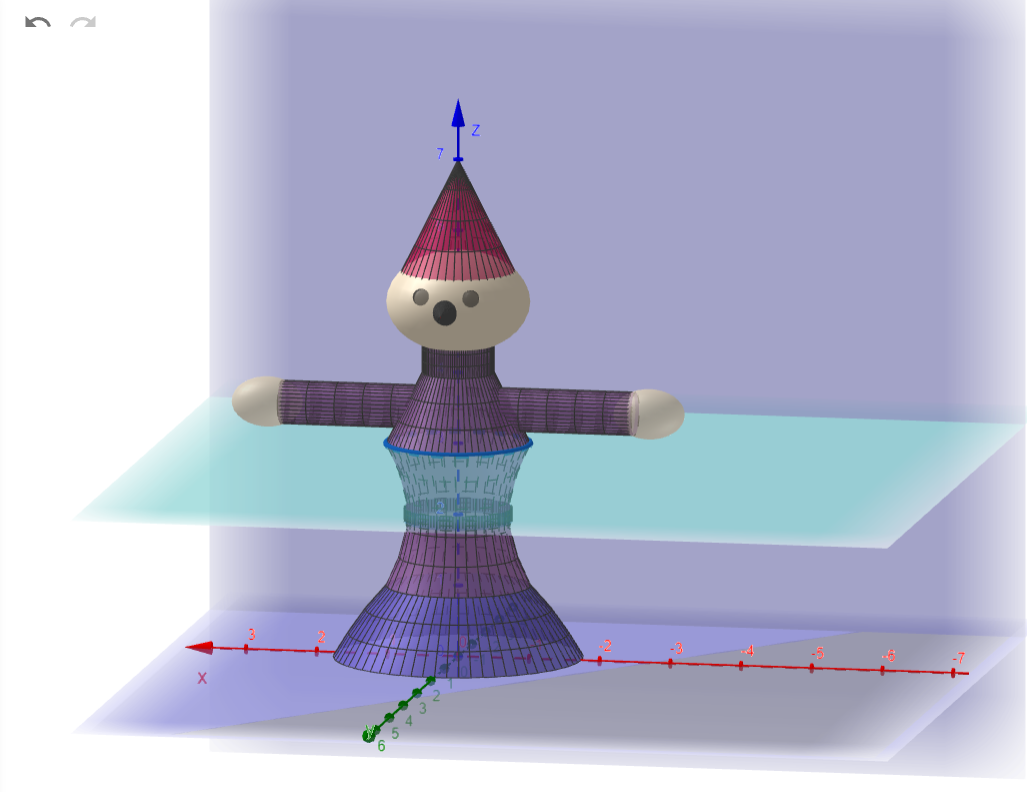
\includegraphics[width=0.48\textwidth]{corteTorsoo.png}\hfill
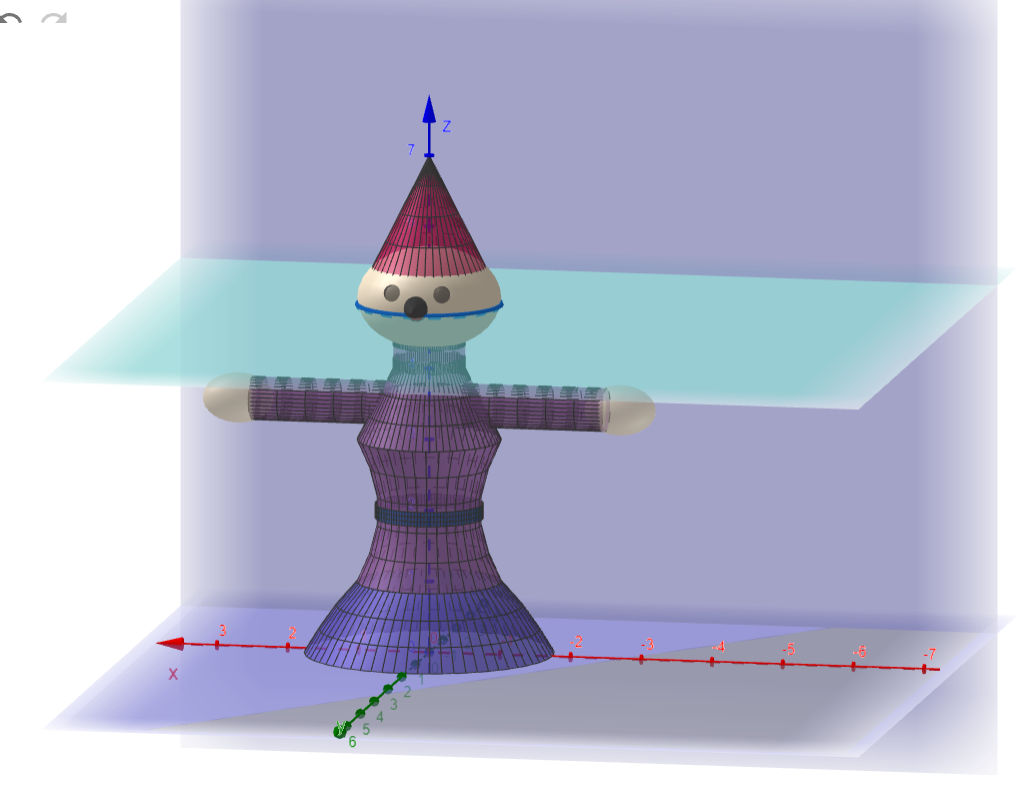
\includegraphics[width=0.48\textwidth]{corteCabeza.png}
\caption{Corte $z=k$ del torso (izquierda) y de la cabeza (derecha): en ambos la curva es un círculo.}
\end{figure}
 
Con el plano $y=0$ se obtienen otras cónicas: en el torso $x^2-\frac{(z-2)^2}{2}=0.5$ (hipérbola), en la cabeza $x^2+\frac{(z-5)^2}{0.5}=1$ (elipse) y en la pelvis $z=1.5-\frac{x^2}{2}$ (parábola).
 
\section{Conclusión}
Todos los cortes horizontales del cuerpo son círculos, por lo que es un sólido de revolución alrededor del eje $z$. Las manos rompen esa simetría porque su corte horizontal es una elipse. Los cortes verticales muestran la hipérbola (torso), la elipse (cabeza) y la parábola (pelvis).
 

\end{document}